\documentclass[runningheads,a4paper]{llncs}

\usepackage{amssymb}
\setcounter{tocdepth}{3}
\usepackage{graphicx}
\usepackage{tikz}
\usetikzlibrary{arrows,chains,positioning,scopes,quotes}

\newcommand{\keywords}[1]{\par\addvspace\baselineskip
\noindent\keywordname\endspace\ignorespaces#1}
\pagestyle{plain}
\setlength\parindent{0pt}

\begin{document}
\def \SystemName {Worlds} % Lol because this shit probably will change.

\mainmatter  % start of an individual contribution

% This needs some work, big time.
\title{\SystemName: A protocol for a distributed MMO}

\author{Ryan Walker\\
				Ryan.cjw@gmail.com\\
				\~wlkr}

\institute{MistyWest}

\maketitle

% - Abstract:  Why, What, How 

% Worlds
%  - Overview
%  - Action Ledger
%  - Transport Hash
%  - Forward Transport hash
%  - World Tranfer
%  - Player Genesis
%  
% Trust
%  - Action ledger traceback
%  - World disconnect

\begin{abstract}
A protocol defining how anyone can join or contribute to a completely unbounded universe could allow the flexibility to organically grow an MMO faster and more efficiently then any proprietary closed system can. This paper will overview a truly limitless yet fair protocol that allows developers to bolt their code into in common universe. 
\end{abstract}

%It is counterintuitive for developers to implement a system for a third party to develop code on their platform. This is simply because maintaining the system holistically would be nearly impossible.
\section{Introduction}
For an open software ecosystem to grow organically there should be outlets for people to contribute. In the context of a massively multiplayer online game these currently do not exist. The fairness and security of the game are entirely dependent on the network forming consensus on what is considered to be the truth. It's trivial to solve this using conventional methods. A server maintains a secure connection with a player and the player pipes his actions to the server. The server then provides ground truth for the network. A distributed system will require a different approach. Blockchains present clear deficiencies, they are too slow, the chain would get too large and they required additional consensus protocols that are still in heavy development. A completely alternate consensus method will now be presented...

\section{Worlds}
\subsection{Overview}
A world, defined as $w_k$, is a node that forms consensus among it's own domain. It's possible for any node in the network to be a world. A world can have up to $?N?$ adjacent worlds determined by itself. Players, defined as $P_k$, can enter a world one of two ways, the first being a \textbf{player genesis}(\ref{PG}), and the second being a \textbf{world transfer} (\ref{WT}). Worlds, just like players have their own RSA key pair. 

%Right now the reader thinks a world is a server

\subsection{Action Ledger}
\label{AL}
An action ledger, defined as $AL(P_{k}, w_k)$, is a chronological list of all the signed actions and reactions that has happened to a player in a world. In order to commit an action a player must concatenate the worlds current nuance with the action then sign and sent to the world. If the action is legal, it is entered into the worlds action ledger for that player. If reactions are to occur to a player, the world must concatenate the players current nuance with the action then sign and sent to the player. Players are required to keep their actions ledger dating back to their genesis, worlds are only required to keep \textbf{transport hashes} (\ref{TH}).

\subsection{Transport Hash}
\label{TH}
A transport hash is simply a secure hash of an action ledger, $h_s(AL(P_{k}, w_k))$, these are secured by the worlds are used to prove a player is presenting an honest action ledger. The transport hash is formed when a player leaves the world. A \textbf{Forward Transport Hash} is just a transport hash kept in a special location. This is explained more in the world transfer section, it is defined as  $h_{sf}(AL(P_{k}, w_k))$

\subsection{World Transfer} 
\label{WT}
There needs to be a secure and fair way for players to transcend worlds. If a player, defined as $P_1$, wants to move from $w_1$ to $w_2$ (Figure \ref{w1tow2}) and then to $w_3$, there is a detailed state machine that honest worlds must adhere to in order to maintain consensus. The network values in this scenario are defined as...

\begin{figure}
\caption{$P_1$ moving from $w_1$ to $w_2$}
\label{w1tow2}
\begin{center}
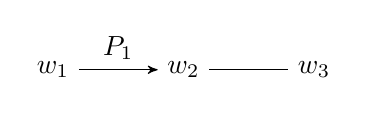
\begin{tikzpicture}[>=stealth']
{[start chain]
\node[on chain] (A) {$w_1$};
\node[on chain,join=by {->,"$P_1$"},right=of A] (B) {$w_2$};
\node[on chain,join=by {-},right=of B] (C) {$w_3$};}
\end{tikzpicture}
\end{center}
\begin{center}
\begin{tabular}{ c|c c c }
& $w_1$ & $w_2$ & $w_3$ \\
\hline 
$h_s(AL(P_1,w_k))$ & $NULL$ & $NULL$ & $NULL$ \\ 
$h_{sf}(AL(P_1,w_k))$ & $NULL$ & $NULL$ & $NULL$ \\ 
Neighbor & $w_2$ & $w_1$ \& $w_3$ & $w_2$\\
\end{tabular}
\end{center}
\end{figure}

\begin{enumerate}
\item First $w_2$ must verify that $P_1$ currently resides in $w_1$, this is done by ensuring $h_{sf}(AL(P_1,w_k)) = NULL$ this is found by sending a signed data request message from $w_2$ to $w_1$ 
\item $w_2$ insures that $w_1$ is adjasent to itself
\item The player presents a $AL(P_1,w_1)$ to $w_2$
\item $w_1$ calculates $h_s(AL(P_1,w_1))$ using the $AL$ on the serverside
\item $w_2$ calculates $h_s(AL(P_1,w_1))$ using the $AL$ provided by $P_1$, the hashes must match
\item (Optional) The Action ledger traceback can be complete
\item $P_1$ is now granted access to $w_2$ and can submit action 
\item $w_1$ must store $h_s(AL(P_1,w_1))$, $AL(P_1,w_1)$ can be deleted
\end{enumerate}

\begin{figure}
\caption{$P_1$ in $w_2$}
\begin{center}
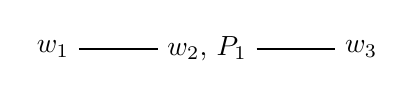
\begin{tikzpicture}[>=stealth']
{[start chain]
\node[on chain] (A) {$w_1$};
\node[on chain,join=by {-},right=of A] (B) {$w_2$, $P_1$};
\node[on chain,join=by {-},right=of B] (C) {$w_3$};}
\end{tikzpicture}
\end{center}
\begin{center}
\begin{tabular}{ c|c c c }
& $w_1$ & $w_2$ & $w_3$ \\
\hline 
$h_s(AL(P_1,w_k))$ & $ h_s(AL(P_1,w_1))$ & $NULL$ & $NULL$ \\ 
$h_{sf}(AL(P_1,w_k))$ & $NULL$ & $NULL$ & $NULL$ \\ 
Neighbor & $w_2$ & $w_1$ \& $w_3$ & $w_2$\\
\end{tabular}
\end{center}
\end{figure}


\begin{figure}
\caption{$P_1$ in $w_3$}
\begin{center}
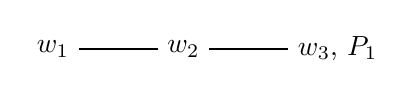
\begin{tikzpicture}[>=stealth']
{[start chain]
\node[on chain] (A) {$w_1$};
\node[on chain,join=by {-},right=of A] (B) {$w_2$};
\node[on chain,join=by {-},right=of B] (C) {$w_3$, $P_1$};}
\end{tikzpicture}
\end{center}
\begin{center}
\begin{tabular}{ c|c c c }
& $w_1$ & $w_2$ & $w_3$ \\
\hline 
$h_s(AL(P_1,w_k))$ & $h_s(AL(P_1,w_1))$ & $h_s(AL(P_1,w_2))$ & $NULL$ \\ 
$h_{sf}(AL(P_1,w_k))$ & $h_s(AL(P_1,w_2))$ & $NULL$ & $NULL$ \\ 
Neighbor & $w_2$ & $w_1$ \& $w_3$ & $w_2$\\
\end{tabular}
\end{center}
\end{figure}

\subsection{Player Genesis} 
\label{PG}
Player Genesis is the creation of a new player, for this to occur a player must digitally sign a genesis package with the current nuance of the world. The player is then instated into the world with all the initial player values set to zero. 

\section{Trust}
The system is not entirely trustless, the neighboring worlds need to trust each other. It's possible for neighboring worlds to have disagreements and still function. For instance, $w_1$ might introduce an item $w_2$ consider to be too powerful, in this case the world can just neglect it's existence, any action presented using that item would be considered illegal and not entered into the action ledger of the $w_1$.

Worlds that have rules that are considered to be completely egregious can be neglected, consider Figure \ref{ThreeWorld}<-WTF? should be fig. 4 

\begin{figure}
\label{ThreeWorld}
\caption{Three adjacent worlds}
\begin{center}
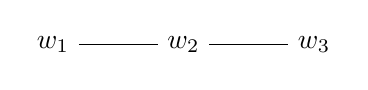
\begin{tikzpicture}[>=stealth']
{[start chain]
\node[on chain] (A) {$w_1$};
\node[on chain,join=by {-},right=of A] (B) {$w_2$};
\node[on chain,join=by {-},right=of B] (C) {$w_3$};}
\end{tikzpicture}
\end{center}
\end{figure}

It's entirely possible that $w_1$ might not agree with the rules of $w_3$. There are two ways of dealing with a dispute like this, either a \textbf{World Disconnect} (\ref{WD}) or \textbf{Action Ledger Traceback}(\ref{ALT}).

\subsection{Action Ledger traceback}
\label{ALT}
Depending on the required security of the world, it may required an Action ledger traceback. If this is requested, the player must provide a list of action ledgers that date back to either the player genesis or to the last entry of the world committing the audit. 

This requests all $h_s{AL(P_k, w_{k:n})}$ from the from $w_k$ to $w_n$. If the hashes match then the players history has been confirmed. It's still entirely possible for the $AL(P_k, w_{k:n})$ to contain actions considered illegal by the world doing the audit. In this case the rewards and actions committed in the offending world are neglected in the world. If you get This will create a phenomenon called \textbf{Action Ledger Fragmentation} (\ref{ALF}) 

\subsection{World Disconnects}
\label{WD}
It's possible a world may issue a disconnect of an adjacent world, this means that players can no longer travel back and fourth through these worlds and they are no longer considered adjacent. If the player resided in the disconnected world this could leave the player stranded in the offending world. It would be logical for the world that issued the disconnect to accept the player back into the world in an earlier state before the player moved into the offending world.

\section{Action Listings}
% Legal Actions - Okay to perform
% Illegal Actions - Not okay to perform anywhere
% Acceptable actions - Okay to perform not in world


\section{Outstanding Issues}
\subsection{Action Ledger Fragmentation}
\label{ALF}


\end{document}
